%% selective-gaussian-blur-body.tex
\paragraph{Filter aus Nutzersicht}
\glqq Im Gegensatz zu den anderen Weichzeichnungsfiltern wirkt der Selektive Gaußsche Weichzeichner nicht auf alle Pixel des Bildes, der Auswahl oder der aktuellen Ebene. Das Filter wirkt nur auf die Pixel, deren Farbe höchstens um einen definierten Wert von der Farbe der Nachbarpixel abweicht. Daher werden Kanten im Bild erhalten.\glqq\footnote{\url{http://docs.gimp.org/	de/plug-in-sel-gauss.html}} 

Das Filter hat zwei Parameter: 
\begin{itemize}
\item \emph{Blur Radius} - beeinflusst maßgeblich die Intensität der Wirkung. Der Radius wird in Pixeln angegeben.
\item \emph{Max. Delta} - stellt die maximale Farbdifferenz im Bereich von 0 bis 255 pro Farbkanal dar. Dieser Wert beeinflusst maßgeblich, wie gut Kanten
gegen das Weichzeichnen geschützt werden.
\end{itemize}


\paragraph{Algorithmus} 
\begin{algorithm}[h]
\caption{Pseudo-Code des \glqq Selective Gaussian Blur\grqq-Algorithmus}
\label{algo:sel-gaussian}
\begin{algorithmic}[1]
\ForAll{$rows$ $\in input$}
	\ForAll{$columns$ $\in input$}
	\ForAll{$color$ $channels$}
		\State $col\_sum \gets 0$
		\ForAll{$y \in blur\_area$}
			\If{$y$ $\not \in input$}
			\State continue
			\EndIf
			\State $row\_sum \gets 0$
			\ForAll{$x \in blur\_area$}
				\If{$x$ $\not \in input$}
				\State{continue}
				\EndIf
				\State{$diff \gets src\_value - area\_value$}
				\If{$diff < delta$}
				\State{continue}
				\EndIf
				\State{$row\_sum \gets coeff * area\_value$}
			\EndFor
			\State{$col\_sum \gets coeff * row\_sum$}
		\EndFor
		\State $dst\_value \gets col\_sum$
	\EndFor
	\EndFor
\EndFor	
\end{algorithmic}
\end{algorithm}

Der Algorithmus funktioniert pixelweise. Jeder Ausgangspixel wird separat bearbeitet, für jeden Pixel werden Werte für Farbkanäle einzeln berechnet. Bei der Berechnung werden benachbarte Pixelwerte mit einer Faltungsmatrix multipliziert, was in \autoref{fig:sgb-grid} dargestellt ist. Die Faltungsmatrix ist 2 * \emph{Radius} groß. Bei der Multiplikation wird jedes benachbarte Pixel mit dem zentralen Eingangspixel verglichen, und wenn die Farbdifferenz kleiner als \emph{Max. Delta} ist, trägt dieses Pixel zum Endergebnis bei. 

Der Quellcode hat zwei äußere Schleifen, die über die Zeilen und Spalten iterieren. Dann wird pro Farbkanal den Pixelwert berechnet, wo man die Eingangswerte mit den Filterkernwerten multipliziert. Die Multiplikation selbst hat auch zwei Schleifen, die über den Filterkern iterieren.   


\begin{figure}
\centering
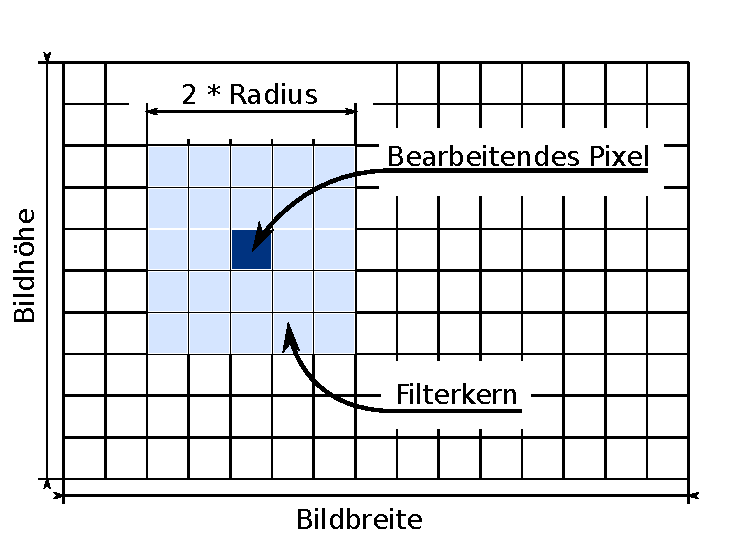
\includegraphics[scale=0.9]{graphs/sgb-grid.pdf}
\caption{Selective Gaussian Blur. Schematische Darstellung}
\label{fig:sgb-grid}
\end{figure} 


\paragraph{Portierung}
Wenn man den GIMP-Code genauer anschaut, sieht man, dass der GIMP-Code zwei Implementierungen hat: normale C-Implementierung und optimierte MMX-Implementierung. Der Quelldatei hat insgesamt 853 Zeilen, 643 davon sind C Code. 

Zuerst haben wir die C-Implementierung untersucht, um zu verstehen, wie genau das Filter funktioniert. Bei der Portierung nach GEGL müssen alle GEGL-Schnittstellen angepasst werden. Worauf auch beachtet werden muss, dass GIMP in Integers rechnet und GEGL in Floats. Der Zugriff zu Bilddaten ist innerhalb eines Tiles, d.h. die Randpixel müssen richtig bearbeitet werden. 

Nach der ersten Portierung kamen die Zeitmessungen. Die Ausführungszeit von GEGL Version war schlechter als die langsame C-Implementierung von GIMP\footnote{Das Testsystem bei der Laufzeitmessung war: Intel® Core i5-2520M Processor, 8 GB RAM, Debian GNU/Linux 7 amd64. Das Testbild war 512x512 Pixel groß. Filterparameter waren: Radius 20, Delta 50.}. Die Laufzeitmessungen sind in (\autoref{fig:sgb-graph-1}) dargestellt.

Die erste Vermutung war, dass das Rechnen in Floats aufwändig ist. Dann haben wir ein Integer Farbformat benutzt, das 8 Bit pro Farbkanal verwendet. Die Berechnung in Integers dauert noch länger.

Der nächste Schritt war die Optimierung. Mithilfe des Intel® VTune Profilers haben wir den Sourcecode nach kritischen Stellen untersucht. Die Optimierung ist ein iterativer Prozess, wo man profiliert, ändert kritische Stelle, danach neu profiliert und vergleicht die Laufzeiten. Sehr große Rolle haben die Schleifenanordnung  und die if-Statements gespielt. Nach der Optimierung haben wir eine neue Codestruktur bekommen. Die Laufzeit nach der Optimierung war 3,179s gegen 3.567s in GIMP Integer und 1.397s in GIMP MMX Versionen. Is es schon besser als GIMP Integerz Implementierung, aber die MMX-Implementierung bleibt trotzdem schnell.

MMX Implementierung verwenden MMX Instruktionen zur Beschleunigung. MMX ist eine Befehlssatzerweiterung mit der SIMD-Architektur. Ein MMX Befehl kann gleichzeitig bis 4 Operanden bearbeiten. Jeder Pixel kann ganz berechnet werden, ohne jeden Farbkanal getrennt zu berechnen. MMX arbeitet nur mit Integers, was für die GEGL-Operation nicht ganz passt. Dafür stehen SSE Instruktionen zur Verfügung. Obwohl der Compiler den Code mithilfe von SSE Instruktionen optimiert, ist diese Optimierung nicht immer die beste.

Der kritischer Abschnitt innerhalb aller Schleifen wurde mit dem SSE Code manuell umgeschrieben. Dies hat einen merkbaren Speedup gegen den Float Code
gezeigt. Die endgültige Ausführungszeiten nach der Optimierung sequentieller Version sind in \autoref{fig:sgb-graph-2} zu sehen. Die GIMP MMX Version bleibt das schnellste sequentielle Implementierung, es lässt sich durch GEGL Overhead erklären.
\begin{figure}
\centering
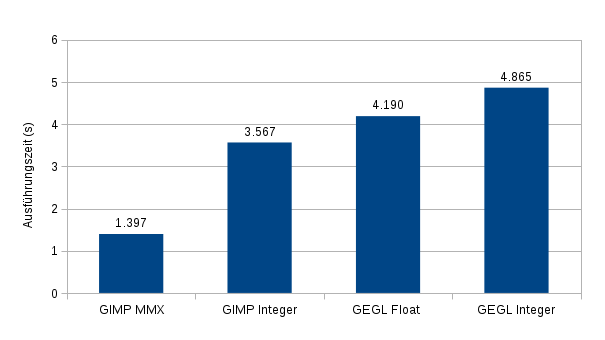
\includegraphics[scale=0.75]{graphs/sgb-graph-1.png}
\caption{Selective Gaussian Blur. Laufzeiten nach der Portierung}
\label{fig:sgb-graph-1}
\end{figure} 

\begin{figure}
\centering
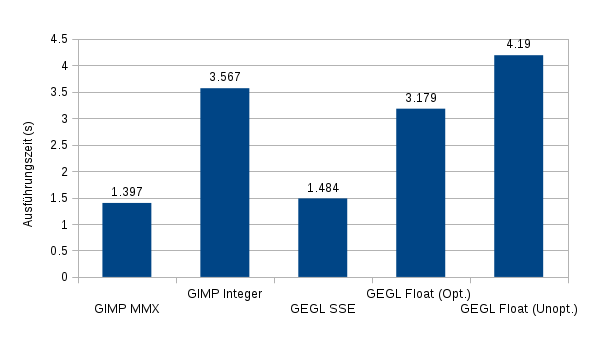
\includegraphics[scale=0.75]{graphs/sgb-graph-2.png}
\caption{Selective Gaussian Blur. Laufzeiten nach der Optimierung}
\label{fig:sgb-graph-2}
\end{figure} 
 

\paragraph{Parallelisierung} 
Der berechnete Pixelwert hängt von benachbarten Pixeln im angegebenen Bereich ab. Da es nur Leseabhängigkeit von konstanten Daten aus dem Eingabebild besteht, könnten alle Pixel gleichzeitig bearbeitet werden.

\subparagraph{OpenMP}
Mit OpenMP ist es sinnvoll die äußerste Schleife zu parallelisieren. Die Parallelisierung wird durch ``\#pragma omp parallel for'' durchgeführt.  Bei diesem Ansatz müssen private Variablen für Threads deklariert werden. Der Pseudo-Code der parallelisierter Version des Filters ist in \autoref{algo:sel-gaussian-par} dargestellt.

\begin{algorithm}[h]
\caption{Pseudo-Code des \glqq Selective Gaussian Blur\grqq-Algorithmus. Parallelisierte Version}
\label{algo:sel-gaussian-par}
\begin{algorithmic}[1]
\State \textcolor{blue}{\#pragma omp parallel for }
\ForAll{$rows$ $\in input$}
	\ForAll{$columns$ $\in input$}
		\ForAll{$y \in blur\_area$}
			\If{$y$ $\not \in input$}
			\State continue
			\EndIf
			\ForAll{$x \in blur\_area$}
				\If{$x$ $\not \in input$}
				\State{continue}
				\EndIf
				\State{\textbf{SSE Code}}
			\EndFor
			\State{$col\_sum \gets coeff * row\_sum$}
		\EndFor
		\State $dst\_value \gets col\_sum$
	\EndFor
\EndFor	
\end{algorithmic}
\end{algorithm}
